% !TeX root = booklet-01.tex
\section{از رابط پردازنده تا \lr{Logic Design}}
\subsection{رابط سطح بالا را پیش از طراحی داخل مشخص کنیم}
رابط جدول \secnum{۱.۹} کتاب، ورودی‌های \code{ph1}، \code{ph2}،
\code{reset} و \code{MemData[7:0]} و خروجی‌های \code{MemWrite}،
\code{Adr[7:0]} و \code{WriteData[7:0]} را دارد
\cite[بخش \secnum{۱.۸.۱}]{weste}.
بازه \code{[7:0]} یعنی هشت بیت از شماره هفت تا صفر؛ تفریق هفت از صفر نیست.
\code{MemWrite} یک سیگنال کنترلی تک‌بیتی است و دو باس داده هرکدام هشت بیت‌اند.

دو ورودی ساعت، دو فاز غیرهم‌پوشان طراحی فیزیکی را بیان می‌کنند؛
نمای \code{CLK} در شکل کلی \lr{Microarchitecture} سطح انتزاع ساده‌تری است.
\code{reset} در متن کتاب \lr{PC} را صفر و کنترل‌کننده را به حالت آغازین می‌برد؛
از این جمله نباید صفرشدن تمام ثبات‌های داده را نتیجه گرفت.

در خواندن، پردازنده آدرس می‌دهد و حافظه \code{MemData} را برمی‌گرداند؛
در نوشتن، آدرس و \code{WriteData} همراه اجازه نوشتن ارائه می‌شوند.
کتاب در این مثال مسیر خواندن و نوشتن داده را جدا نگه می‌دارد.
ترکیب آن‌ها در باس دوطرفه ممکن است، ولی به کنترل جهت و جلوگیری از
راه‌اندازی متضاد نیاز دارد و تغییر ساده نام سیم نیست.
رابط حافظه دارای \lr{Handshake} یا چرخه انتظار، خارج از قرارداد ساده این مثال است.

\subsection{\lr{Wordslice}، \lr{Bitslice} و \lr{Zipper}}
در \lr{Wordslice}، یک واحد چندبیتی کامل مانند \lr{MUX} هشت‌بیتی یا ثبات
هشت‌بیتی را یک ستون می‌بینیم. در \lr{Bitslice}، یک ردیف شامل یک بیت
از هر واحد و اتصال‌های همان بیت است
\cite[بخش \secnum{۱.۸.۲} و شکل \secnum{۱.۵۷}]{weste}.
این دو، دو روش نگاه به سازمان فیزیکی و منطقی مسیر داده‌اند؛
یکی به معنی «هشت مدار متفاوت» و دیگری به معنی «بدون سیم بین بیت‌ها» نیست.

برای یک \lr{MUX} هشت‌بیتی، هشت \lr{MUX} تک‌بیتی داریم که همگی یک
انتخاب مشترک می‌گیرند. مدار بافر و تولید مکمل انتخاب را می‌توان در ناحیه مشترکی
قرار داد؛ کتاب به این ناحیه \lr{Zipper} می‌گوید.
این کار می‌تواند از تکرار هشت مدار تولید مکمل جلوگیری کند،
ولی طول سیم و بار مشترک باید بررسی شود. جای میانی یا کناری این ناحیه، تصمیم فیزیکی است.

در جمع‌کننده، \lr{Carry} از یک بیت به بیت دیگر می‌رود؛
در تشخیص صفر، خروجی بیت‌ها باید با هم ترکیب شوند.
پس همه اتصال‌ها صرفاً محلی و همه \lr{Bitslice}ها الزاماً مستقل و یکسان نیستند.
در همین مثال، کتاب \lr{Datapath} منظم را مناسب طراحی تکرارشونده و کنترل‌کننده
کم‌قاعده‌تر را مناسب توصیف انتزاعی و ابزار خودکار معرفی می‌کند.

\subsection{سلسله‌مراتب باید قابل ردیابی بماند}
شکل \ref{fig:logic-hierarchy} بخشی از سلسله‌مراتب کتاب را فشرده بازنمایی می‌کند.
\lr{Leaf Cell} پایین‌ترین بلوک در سطحی است که فعلاً به جزئیات آن وارد نمی‌شویم؛
ممکن است در سطح مدار خودش از چند ترانزیستور تشکیل شده باشد.

\begin{figure}[ht]
\centering
\begin{latin}
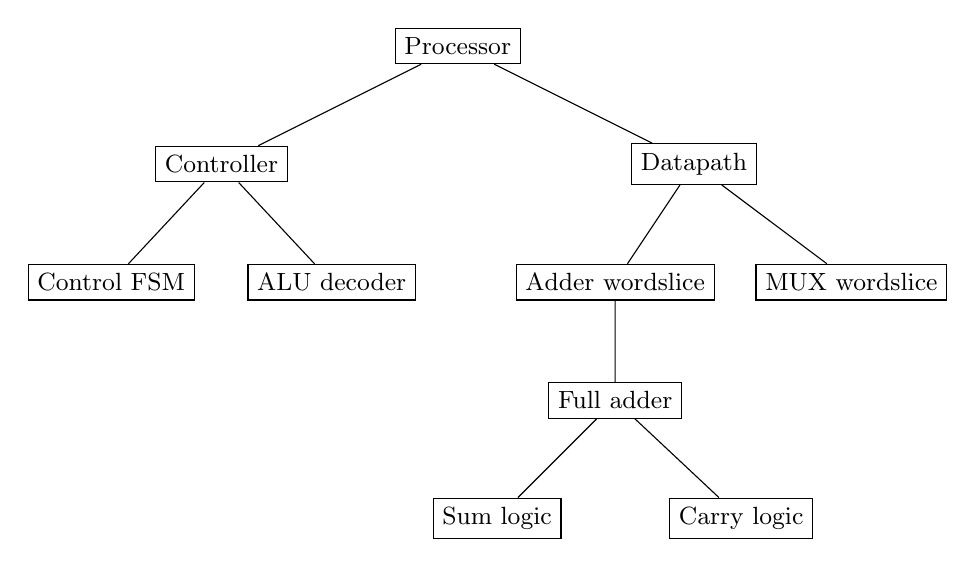
\begin{tikzpicture}[font=\small]
\node[draw] (top) at (0,3) {Processor};
\node[draw] (ctrl) at (-3,1.5) {Controller};
\node[draw] (data) at (3,1.5) {Datapath};
\node[draw,align=center] (fsm) at (-4.4,0) {Control FSM};
\node[draw,align=center] (dec) at (-1.6,0) {ALU decoder};
\node[draw] (add) at (2,0) {Adder wordslice};
\node[draw] (mux) at (5,0) {MUX wordslice};
\node[draw] (fa) at (2,-1.5) {Full adder};
\draw (top)--(ctrl) (top)--(data) (ctrl)--(fsm) (ctrl)--(dec);
\draw (data)--(add) (data)--(mux) (add)--(fa);
\node[draw] (sum) at (0.5,-3) {Sum logic};
\node[draw] (carry) at (3.6,-3) {Carry logic};
\draw (fa)--(sum) (fa)--(carry);
\end{tikzpicture}
\end{latin}
\caption{سلسله‌مراتب آموزشی فشرده بر پایه شکل \secnum{۱.۵۸} کتاب \cite{weste}؛
این شاخه‌ها تمام بلوک‌های پردازنده را فهرست نمی‌کنند.}
\label{fig:logic-hierarchy}
\end{figure}

سلسله‌مراتب منطقی، مداری و فیزیکی الزاماً یکسان نیست، اما تفاوت زیاد آن‌ها
تطبیق و \lr{Verification} را دشوار می‌کند.
مثلاً حافظه در نمای بالا یک بلوک است و در سطح مدار، آرایه و \lr{Decode} و مسیرهای
خواندن دارد. باید معلوم باشد هر بلوک در نمای دیگر کجا و چگونه پیاده شده است
\cite[بخش \secnum{۱.۸.۳}]{weste}.

\section{خواندن مقدماتی \lr{HDL}}
\subsection{توصیف سخت‌افزار با برنامه ترتیبی یکسان نیست}
\lr{Hardware Description Language (HDL)} مانند \lr{Verilog}،
\lr{SystemVerilog} یا \lr{VHDL} برای توصیف مدار به کار می‌رود.
دو سبک کلی، \lr{Structural} برای نمونه‌سازی و اتصال بلوک‌ها و
\lr{Behavioral} برای بیان رفتار وجود دارد
\cite[بخش \secnum{۱.۸.۴}]{weste}\cite[اسلایدهای ۱۹ و ۲۰]{intro}.
کتاب از برخی سازه‌های \lr{SystemVerilog} مانند \code{logic} استفاده می‌کند؛
کد آموزشی این بخش نیز با همین خانواده نحو نوشته شده است.

در کد سخت‌افزار، دو نمونه گیت هم‌زمان وجود دارند و برای فعالیت منتظر اجرای
ترتیبی دو خط نرم‌افزاری نمی‌مانند. دستور \code{assign} رابطه پیوسته خروجی
با ورودی‌ها را توصیف می‌کند؛ وقتی ورودی تغییر کند، خروجی مدل مطابق رابطه به‌روزرسانی می‌شود.
برای مدار دارای حالت و ساعت، باید عنصر ذخیره و رویداد ثبت نیز توصیف شود؛
کد نمونه زیر فقط \lr{Combinational} است.

\subsection{رابطه \lr{Full Adder} را پیش از کد استخراج کنیم}
سه بیت \(a,b,c_{\mathrm{in}}\) را جمع می‌کنیم؛ خروجی جمع تک‌بیتی \(s\)
و نقلی \(c_{\mathrm{out}}\) است.
از شمارش تعداد یک‌ها، رابطه حسابی زیر حاصل می‌شود:
\begin{equation}\label{eq:hdl-fulladder-number}
a+b+c_{\mathrm{in}}=s+2c_{\mathrm{out}}.
\end{equation}
جمع این رابطه حسابی است، نه \lr{OR}؛ سمت چپ می‌تواند صفر تا سه باشد.
\(s\) وقتی تعداد یک‌ها فرد باشد یک می‌شود، پس \lr{XOR} سه ورودی است.
نقلی وقتی دست‌کم دو ورودی یک باشند یک می‌شود؛ بنابراین با عملگرهای منطقی:
\begin{equation}\label{eq:hdl-fulladder}
s=a\oplus b\oplus c_{\mathrm{in}},\qquad
c_{\mathrm{out}}=ab+ac_{\mathrm{in}}+bc_{\mathrm{in}}.
\end{equation}
در رابطه دوم، \(+\) به معنی \lr{OR} است.
برای نمونه \((a,b,c_{\mathrm{in}})=(1,1,0)\)، تعداد یک‌ها دو است؛
پس \(s=0\) و \(c_{\mathrm{out}}=1\).
این همان منطق جمع و نقلی مثال شکل \secnum{۱.۵۹} کتاب است.

\subsection{کد یک‌بیتی و تفسیر هر بخش}
کد زیر بازنویسی آموزشی رفتار جمع‌کننده است:
\begin{latin}
\small
\begin{verbatim}
module fulladder(
    input  logic a, b, cin,
    output logic sum, cout
);
    assign sum  = a ^ b ^ cin;
    assign cout = (a & b) | (a & cin) | (b & cin);
endmodule
\end{verbatim}
\end{latin}
\code{module} مرز بلوک و \code{input/output} جهت پایه‌ها را تعیین می‌کند.
\code{logic} نوع سیگنال است و به‌تنهایی وجود ثبات فیزیکی را اثبات نمی‌کند.
در این مثال، \code{\textasciicircum} عمل \lr{XOR}، \code{\&} عمل \lr{AND} و
\code{|} عمل \lr{OR} بیت‌به‌بیت است. پرانتزهای نقلی، گروه‌بندی رابطه را روشن می‌کنند.
دو \code{assign} هم‌زمان منطق دو خروجی را تعریف می‌کنند؛
نباید ترتیبشان را مانند دو خط تغییر متغیر در برنامه \lr{Fibonacci} تفسیر کرد.

\subsection{هشت بیت با اتصال نقلی میان مرحله‌ها}
در \lr{Ripple Carry Adder}، نقلی خروجی بیت \(i\) ورودی بیت \(i+1\) می‌شود.
\(c_0\) نقلی اولیه و \(c_8\) نقلی نهایی برای هشت بیت است.
همه سلول‌ها هم‌زمان وجود دارند، ولی در مدار واقعی تغییر نقلی باید از مسیر گیت‌ها عبور کند؛
همین مسیر بر تاخیر اثر دارد. این مثال، ارتباط \lr{Hierarchy} و \lr{Regularity} را نشان می‌دهد.

\begin{latin}
\small
\begin{verbatim}
module adder8(
    input  logic [7:0] a, b,
    input  logic cin,
    output logic [7:0] sum,
    output logic cout
);
    logic [8:0] c;
    assign c[0] = cin;
    for (genvar i = 0; i < 8; i++) begin : bit_slice
        fulladder fa(
            .a(a[i]), .b(b[i]), .cin(c[i]),
            .sum(sum[i]), .cout(c[i+1])
        );
    end
    assign cout = c[8];
endmodule
\end{verbatim}
\end{latin}
حلقه با \code{genvar} هنگام بسط ساختار، هشت نمونه مدار تولید می‌کند؛
به معنی اجرای یک جمع تک‌بیتی در هشت چرخه نیست.
نه بیت سیم نقلی داریم، چون برای هشت سلول یک نقلی قبل از اول و یک نقلی بعد از آخر لازم است.
اتصال نام‌دار مانند \code{.cin(c[i])} پایه نمونه را به سیگنال بیرونی وصل می‌کند.

\textbf{مثال عددی.} برای \(a=15\)، \(b=1\) و \(c_{\mathrm{in}}=0\)،
چهار بیت پایین جمع صفر و نقلی به بیت چهارم می‌رسد، پس نتیجه ۱۶ است.
برای \(a=255,b=1\)، هشت بیت خروجی صفر و نقلی نهایی یک است.
اگر فقط هشت بیت پایین مصرف شوند، مقدار ۲۵۶ در آن‌ها جا نمی‌شود؛
نقلی و سرریز علامت‌دار نیز مفاهیم یکسانی نیستند.

\subsection{مرز \lr{Simulation}، \lr{Synthesis} و صحت}
\lr{Logic Simulation} رفتار مدل را برای ورودی و زمان‌بندی تعریف‌شده بررسی می‌کند.
\lr{Synthesis} سازه‌های قابل سنتز را به شبکه سلول‌ها نگاشت می‌کند؛
\lr{Place and Route} اجزا و سیم‌ها را در هندسه قرار می‌دهد.
همه سازه‌های \lr{HDL} قابل سنتز نیستند؛ مثلاً کارهای فایل‌خوانی
\lr{Testbench} لزوماً مدار موردنظر برای تراشه نمی‌سازند
\cite[صفحه چاپی ۴۱]{weste}.

برابر بودن رابطه حسابی با مدل منطقی، تاخیر فیزیکی، توان یا قابلیت ساخت را
تایید نمی‌کند. همچنین اجرای چند ورودی به‌تنهایی پوشش همه ورودی‌ها را ثابت نمی‌کند.
در این بخش می‌توان تمام هشت حالت \lr{Full Adder} و همه ترکیب‌های جمع هشت‌بیتی
را در مدل رفتاری بررسی کرد؛ نتیجه آن باید جدا از \lr{Compile} یا \lr{Simulation} خود \lr{HDL} گزارش شود.

\section{تمرین‌های جمع‌بندی و پاسخ}
\subsection{پرسش‌ها}
\begin{enumerate}
\item چرا چهار چرخه \lr{Fetch} با هشت‌بیتی بودن داده ناسازگار نیست؟
\item اگر دستور شاخه در آدرس ۲۰ باشد و ثابت آن منفی دو باشد،
مقصد شاخه گرفته‌شده در مدل هشت‌بیتی چیست؟
\item چرا در برنامه کتاب، مقدار دوم حلقه از \code{f1} تازه استفاده می‌کند؟
\item آیا جدول \lr{FSM} رسم‌شده، به‌تنهایی اجرای \code{ADDI} برنامه را پیاده می‌کند؟
\item تفاوت \code{ALUOp} و \code{ALUControl} و تفاوت \lr{Wordslice} و \lr{Bitslice} چیست؟
\item چرا حلقه \code{genvar} در جمع‌کننده به معنی هشت چرخه اجرای نرم‌افزاری نیست؟
\end{enumerate}

\subsection{پاسخ‌های تشریحی}
\begin{enumerate}
\item عرض دستور ۳۲ بیت و عرض انتقال حافظه هشت بیت است؛
در هر چرخه یک‌چهارم دستور خوانده می‌شود. عرض داده عملیاتی جداست.
\item \lr{PC} پس از \lr{Fetch} برابر ۲۴ است و جابه‌جایی
\(4\times(-2)=-8\)، پس مقصد ۱۶ می‌شود.
\item دستورها ترتیبی‌اند؛ با مقادیر قدیمی \(a,b\)،
ابتدا \(a+b\) و سپس \((a+b)-b=a\) تولید می‌شود.
\item خیر؛ حالت‌های آن در نمودار کتاب به‌عنوان تمرین حذف شده‌اند.
صحت ردگیری رفتاری برنامه، کامل بودن مدار کنترل رسم‌شده را اثبات نمی‌کند.
\item اولی فرمان کلی \lr{FSM} به \lr{Decode} محلی است و دومی انتخاب نهایی عمل \lr{ALU}؛
\lr{Wordslice} یک واحد چندبیتی و \lr{Bitslice} یک ردیف از بیت‌های متناظر واحدهاست.
\item حلقه در بسط ساختار، چند نمونه سخت‌افزار می‌سازد؛
هیچ حالت و شمارنده چرخه‌ای در کد این جمع‌کننده تعریف نشده است.
\end{enumerate}

\subsection{آمادگی برای ادامه فصل}
اکنون باید بتوانید تفاوت سطح و دامنه طراحی، نقش رابط، معنای حالت پردازنده،
مسیر دستور از حافظه تا اجرا، کدگذاری یک دستور و رفتار یک نمونه ساده \lr{HDL} را توضیح دهید.
بخش‌های \secnum{۱.۹} تا \secnum{۱.۱۲} این مسیر را به مدار، طراحی فیزیکی،
\lr{Verification} و ساخت و آزمون تراشه پیوند خواهند داد.
